\documentclass{dissert}
\usepackage[T2A]{fontenc}
\usepackage[utf8]{inputenc}
\usepackage[english,russian]{babel}

\usepackage{fullpage}
\usepackage{lastpage}
\usepackage{enumerate}

\usepackage[all]{xy}
% colors
\usepackage{xcolor}
\definecolor{darkgreen}{rgb}{0.0, 0.2, 0.13}
\definecolor{darkcyan}{rgb}{0.0, 0.55, 0.55}

\usepackage{geometry}
\geometry{left=2.5cm}
\geometry{right=1.0cm}
\geometry{top=2.0cm}
\geometry{bottom=2.0cm}
\renewcommand{\baselinestretch}{1.0}

\newcommand{\paragraph}[1]{\noindent\textbf{#1}\quad}


%https://tex.stackexchange.com/questions/163451/total-number-of-citations
\usepackage{totcount}
\newtotcounter{citnum} %From the package documentation
\def\oldbibitem{} \let\oldbibitem=\bibitem
\def\bibitem{\stepcounter{citnum}\oldbibitem}

\makeatletter
\long\def\@makecaption#1#2{%
  \vskip\abovecaptionskip
  \sbox\@tempboxa{#1.~#2}%
  \ifdim \wd\@tempboxa >\hsize
    #1.~#2\par
  \else
    \global \@minipagefalse
    \hb@xt@\hsize{\hfil\box\@tempboxa\hfil}%
  \fi
  \vskip\belowcaptionskip}
\makeatother

\reversemarginpar

\renewcommand{\contentsname}{Содержание}
\renewcommand{\contentsdesc}{Стр.}
\renewcommand{\chaptername}{Глава}

%%% Библиография %%%
\makeatletter
\bibliographystyle{utf8gost71u}     % Оформляем библиографию по ГОСТ 7.1 (ГОСТ Р 7.0.11-2011, 5.6.7)
\makeatother


% Нужные мне пакеты
\usepackage{amsthm}
\usepackage{graphicx}
\usepackage{amssymb}
\usepackage{amsmath}
\usepackage{graphicx}
\usepackage{subfig}
\usepackage{caption}
\usepackage{color}
\usepackage{bm}
\usepackage{tabularx}
\usepackage{url}
\usepackage{multirow}

\newtheorem{theorem}{Теорема}
\newtheorem{lemma}[theorem]{Лемма}
\newtheorem{definition}{Определение}

\usepackage{comment}
\usepackage{rotating}

\usepackage{autonum}

\begin{document}

\begin{titlepage}
%\begin{center}
%\textsc{МОСКОВСКИЙ ФИЗИКО-ТЕХНИЧЕСКИЙ ИНСТИТУТ (ГОСУДАРСТВЕННЫЙ УНИВЕРСИТЕТ)}\\
%\end{center}
%\vspace{1.5cm}
\begin{flushright}
{На правах рукописи}
\end{flushright}
\vspace{1.5cm}
\begin{center}
{Грабовой Андрей Валериевич}
\par
\vspace{2cm}
\textsc{Априорное распределение параметров \\в задачах выбора моделей глубокого обучения}
\par
\vspace{2cm}
{05.13.17~--- Теоретические основы информатики}
\par
\vspace{2cm}
{АВТОРЕФЕРАТ\\
диссертации на соискание ученой степени\\
кандидата физико-математических наук}
\end{center}
\par
\vspace{3.5cm}
\begin{center}
{Москва~--- 2022}
\end{center}
\end{titlepage}

%\clearpage\maketitle
\setcounter{page}{2}
%\pretolerance=10000
%\thispagestyle{empty}
\noindent {Работа выполнена на Кафедре интеллектуальных систем Федерального государственного автономного образовательного учреждения высшего образования <<Московский физико-технический институт (национальный исследовательский университет)>>.

\vspace{0.1cm}

%\begin{sloppy}
%\fontdimen2\font=3pt

\vskip1ex\noindent
\begin{tabularx}{\linewidth}{@{}lX@{}}
  Научный руководитель: & \textbf{Стрижов Вадим Викторович}\\
  & доктор физико-математических наук, Федеральный исследовательский~центр <<Информатика и управление>> Российской академии наук, отдел интеллектуальных систем, ведущий научный сотрудник.
  \\[2pt]
  Официальные оппоненты: & \textbf{Кузнецов Сергей Олегович}\\
  & доктор физико-математических наук, Федеральное государственное автономное образовательное учреждение высшего образования «Национальный исследовательский университет «Высшая школа экономики», заведующий международной лабораторией интеллектуальных систем и структурного анализа.\\[2pt]
  & \textbf{Панов Максим Евгеньевич}\\
  & кандидат физико-механических наук, Автономная некоммерческая образовательная организация высшего образования «Сколковский институт науки и технологий», старший преподаватель.\\[2pt]
  Ведущая организация: & Федеральное государственное бюджетное образовательное учреждение высшего образования <<Московский государственный университет имени М.В.Ломоносова>>.
\end{tabularx}
\vskip2ex\noindent

\vspace{0.2cm}
\noindent Защита состоится~21~апреля 2022 года~в~14:00 на~заседании диссертационного совета Д 002.073.05 при Федеральном исследовательском центре <<Информатика и управление>> Российской академии наук (ФИЦ~ИУ~РАН) по адресу: 119333, г.\,Москва, ул.\,Вавилова, д.\,40.

\vspace{0.2cm}
\noindent С диссертацией можно ознакомиться в библиотеке Федерального государственного учреждения Федеральный исследовательский центр <<Информатика и управление>> Российской академии наук и на сайте http://www.frccsc.ru/

\vspace{0.2cm}
\noindent Автореферат разослан  \qquad \qquad \qquad \qquad 2022 года.

\vspace{0.3cm}
\noindent Ученый секретарь\\
диссертационного совета Д 002.073.05\\
к.т.н.
\hspace{12cm} И.\,А.\;Рейер
}

\clearpage


%%%%%%%%%%%%%%%%%%%%%%%%%%%%%%%%%%%%%%%%%%%%%%%%%%%%%%%%%%%%%%%%%%%%%%%%

\pretolerance=-1

%\setcounter{page}{0}

\section*{Общая характеристика работы}
\textbf{Актуальность темы.}
Построение и выбор оптимальной структуры нейронной сети является вычислительно сложной процедурой~(Sutskever: 2014), которая значимо влияет на итоговое качество модели. 
При этом большинство параметров модели перестают значимо изменяться уже после небольшого числа итераций алгоритма оптимизации~(Chunyan: 2016).
Своевременное определение начала сходимости параметров существенно снижает вычислительные затраты на обучение моделей с большим числом параметров.
Примерами таких моделей являются AlexNet~(Krizhevsky: 2012), VGGNet~(Simonyan: 2014), ResNet~(Kaiming: 2015), BERT(Devlin: 2018, Vaswani: 2017), mT5~(Linting: 2021), GPT3~(Brown: 2020).
Рост числа параметров моделей глубокого обучения влечет снижение интерпретируемости ответов этих моделей~(Ivakhnenko: 1994).
Проблема с неинтерпретируемыми моделями рассматривается в классе задач по состязательным атакам~(Zheng: 2020).

Проблемой моделей с большим числом параметров является увеличение вычислительной сложности.
Использование избыточно сложных моделей с большим числом неинформативных параметров является препятствием для использования глубоких сетей на мобильных устройствах в режиме реального времени. \textit{Сложность модели} определяется числом настраиваемых параметров модели.
Для снижения числа параметров в литературе рассматривается метод дистилляции модели на основе предсказаний модели учителя~(Hinton: 2015, Vapnik: 2015, Lopez: 2016).
Сложная модель с большим числом параметров называется~\textit{учитель}. Модель учителя дистиллируется в менее сложную модель с малым числом параметров, которая называется~\textit{ученик}.
Методы дистилляции моделей глубокого обучения введены в работах Дж.\,Е. Хинтона и В.\,Н. Вапником~(Hinton: 2015, Vapnik: 2015, Lopez: 2016).
Предлагается использовать предсказания модели учителя для повышения качества ученика.
В работе~(Vapnik: 2015) В.\,Н. Вапником вводится понятие привилегированной информации. Оно использует дополнительную информацию о данных в момент обучения модели.
Работа~(Lopez: 2016) объединяет идеи дистилляции~(Hinton: 2015) с идеями привилегированного обучения~(Vapnik 2015). Предлагается метод дистилляции учителя в модель ученика в случае, когда признаковое описания объектов не совпадает.
В~(Lopez: 2016) решается двухэтапная задача. На первом этапе строится модель учителя с расширенным признаковым описанием.
На втором этапе при помощи дистилляции~(Hinton: 2015) обучается ученик в исходном признаковом описании.
В работе Дж.\,Е. Хинтона~(Hinton: 2015) поставлены эксперименты по дистилляции моделей глубокого обучения для задачи классификации.
Первый эксперимент анализирует выборку MNIST. Он показывает, что предложенный метод дистилляции позволяет построить нейросетевую модель меньшей сложности на основе модели большей сложности.
Второй эксперимент анализирует метод дистилляции ансамбля моделей в одну нейросетевую модель для решения задачи распознания речи. В работе~(Hinton: 2015) проводится сравнение дистилляции с моделью смеси экспертов.
Дальнейшие работы по дистилляции моделей глубокого обучения исследуют методы, использующие информации о значениях параметров модели учителя, для оптимизации параметров модели ученика. В~(Zehao: 2017) предлагается метод передачи селективности~(Tatarchuk: 2014) нейрона, минимизирующий специальную функцию потерь. Эта функция основывается на максимизация среднего описания между выходами слоев модели учителя и модели ученика. В рамках вычислительного эксперимента сравнивалось качество базовой дистилляции с предложенным методов на примере выборок CIFAR и ImageNet.

Дистилляция моделей глубокого обучения предполагает, что архитектура модели ученика уже известна. Для выбора архитектуры модели ученика предлагается использовать методы прореживания нейросетевых моделей. В работах~(Maclarin: 2015, Luketina: 2015) предлагается использовать алгоритма градиентного спуска для оптимизации сети. В~(Molchanov: 2017) используются байесовские методы~(Neal: 1995) оптимизации параметров нейронных сетей. Существуют методы поиска оптимальной структуры используя удаления параметров сложной модели~(Cun: 1990, Louizos: 2017, Graves: 2011). В работе~(Cun: 1990) предлагается удалять наименее~\textit{релевантные} параметры на основе значений первой и второй производных функции ошибки. В~(Grabovoy: 2019) предложен метод определения релевантности параметров аппроксимирующих моделей при помощи метода Белсли. \textit{Релевантность} параметров в работе~(Grabovoy: 2019) определяется на основе ковариационной матрицы параметров модели.
Другим примером задания порядка на множестве параметров служит $l_1$-регуляризация~(Tibshirani: 1996) и регуляризация ElasticNet~(Hastie: 2005) для линейных моделей.
Порядок, заданный на множестве значений коэффициентов регуляризации, индуцирует порядок на множестве признаковых описаний и указывает на важность признаков.
В случае нейросетей для регуляризации параметров используется метод исключения параметров~(Srivastava: 2014, Molchanov: 2017).
Он также задает порядок на множестве параметров модели.

Порядок на множестве параметров нейросети используется не только для удаления наименее релевантных параметров, а и для фиксации параметров в процессе их оптимизации. Работа~(Grabovoy: 2020) посвящена оптимизации структуры нейронной сети, а также выбору параметров, которые фиксируются после некоторой итерации градиентного метода. 


\vspace{0.5cm}
\textbf{Цели работы.}
\vspace{0.2cm}
\begin{enumerate}
\item Предложить байесовский метод выбора моделей с использованием модели учителя с привилегированной и накопленной информацией.
\item Предложить метод назначения априорного распределения параметров модели ученика с использованием апостериорного распределения параметров модели учителя.
\item Предложить вероятностную интерпретацию дистилляции моделей глубокого обучения.
\item Предложить метод использования экспертной информации о решаемой задаче прогнозирования при построении априорного распределения параметров.
\item Предложить метод назначения релевантности параметров моделей глубокого обучения для выбора модели машинного обучения.
\end{enumerate}

\vspace{0.5cm}
\textbf{Методы исследования.} Для достижения поставленных целей используются методы вариационного байесовского вывода~(MacKay: 2002, Bishop: 2006), вероятностные~(Shiriyaev: 1980) методы анализа моделей глубокого обучения, статистические методы~(Kobzar: 2012, Bishop: 2006) анализа распределений параметров моделей глубокого обучения.

\vspace{0.5cm}
\textbf{Основные положения, выносимые на защиту.}
\vspace{0.3cm}
\begin{enumerate}
    \item Предложен байесовский метод выбора моделей с использованием модели учителя с привилегированной и накопленной информацией.
    \item Доказаны теоремы о свойствах дистилляции, 
    \begin{itemize}
        \item[---] \emph{теоремы об эквивалентности} для дистилляции моделей в случае задачи регрессии и классификации,
        \item[---] \emph{теоремы о виде априорного распределения} параметров модели ученика в байесовской дистилляции.
    \end{itemize}
    \item Предложен метод выравнивания вероятностных пространств параметров. Предложен метод выбора априорного распределения параметров модели ученика с использованием апостериорного распределения параметров модели учителя для случаев
    \begin{itemize}
        \item[---] различных размерностей пространств параметров отдельных слоев,
        \item[---] различного числа слоев нескольких моделей.
    \end{itemize}
    \item Предложены методы задания порядка на множестве параметров моделей
    \begin{itemize}
        \item[---] на основе корреляции параметров,
        \item[---] на основе оценки скорости сходимости параметров.
    \end{itemize}
    \item Предложена вероятностная интерпретации дистилляции моделей глубокого обучения. Исследованы свойства дистилляции моделей глубокого обучения.
\end{enumerate}

\vspace{0.5cm}
\textbf{Научная новизна.} Разработаны новые подходы к назначению априорного распределения параметров моделей. Предложен метод назначения априорного распределения используя экспертную информацию о задаче. Предложены методы задания порядка на множестве параметров нейросетевых моделей на основе анализа мультиколлиниорности параметров и скорости их сходимости. Предложено вероятностное обобщение дистилляции моделей. Предложено байесовское обобщение дистилляции моделей глубокого обобщения.

\vspace{0.5cm}
\textbf{Теоретическая значимость.} Диссертационная работа носит теоретический характер. В работе проводится теоретический анализ методов снижения размерности пространства параметров нейросетевых моделей. Доказаны~\emph{теоремы об эквивалентности} для дистилляции моделей в случае задачи регрессии и классификации. Доказаны~\emph{теоремы об априорном} распределения модели для байесовской дистилляции.

\vspace{0.5cm}
\textbf{Практическая значимость.} Предложенные в работе методы предназначены для построения моделей глубокого обучения в прикладных задачах регрессии и классификации; снижения пространства параметров моделей глубокого обучения; использования экспертной информации для построения моделей; дистилляции параметрических моделей на основе выравнивания архитектур.

\vspace{0.5cm}
\textbf{Степень достоверности и апробация работы.} Достоверность результатов подтверждена математическими доказательствами, экспериментальной проверкой полученных методов на реальных задачах выбора моделей глубокого обучения; публикациями результатов исследования в рецензируемых научных изданиях, в том числе рекомендованных ВАК. Результаты работы докладывались и обсуждались на следующих научных конференциях.
\begin{enumerate}
    \item Задача обучения с экспертом для построения интерпретируемых моделей машинного обучения, Международная конференция <<Интеллектуализация обработки информации>>, 2020.
    \item Привилегированная информация и дистилляция моделей, Всероссийская конференция <<63-я научная конференция МФТИ>>, 2020.
    \item Введение отношения порядка на множестве параметров нейронной сети, Всероссийская конференция <<Математические методы распознавания образов ММРО>>, 2019.
    \item Анализ априорных распределений в задаче смеси экспертов, Всероссийская конференция <<62-я научная конференция МФТИ>>, 2019.
    \item Поиск оптимальной модели при помощи алгоритмов прореживания, Всероссийская конференция <<61-я научная конференция МФТИ>>, 2018.
    \item Автоматическое определение релевантности параметров нейросети, Международная конференция <<Интеллектуализация обработки информации>>, 2018.
\end{enumerate}

Работа поддержана грантами Российского фонда фундаментальных исследований:

\begin{enumerate}
    \item[1)] 19-07-00875, Развитие методов автоматического построения и выбора вероятностных моделей субоптимальной сложности в задачах глубокого обучения,
    \item[2)] 19-07-01155, Развитие теории порождения моделей локальной аппроксимации для классификации сигналов носимых устройств,
    \item[3)] 19-07-00885, Выбор моделей в задачах декодирования временных рядов высокой размерности.
\end{enumerate}

\vspace{0.5cm}
\textbf{Публикации по теме диссертации.} Основные результаты по теме диссертации изложены в 6 печатных изданиях в журналах, рекомендованных ВАК.

\vspace{0.5cm}
\textbf{Личный вклад.} Все приведенные результаты, кроме отдельно оговоренных случаев, получены диссертантом лично при научном руководстве д.ф.-м.н. В. В. Стрижова.

\vspace{0.5cm}
\textbf{Структура и объем работы.} Диссертация состоит из оглавления, введения, шести разделов, заключения, списка иллюстраций, списка таблиц, перечня основных обозначений и списка литературы из~$99$ наименований. Основной текст занимает~$124$ страницы.

\section*{Основное содержание работы}
Во~\textbf{введении} обоснована актуальность диссертационной работы, сформулированы цели и методы исследования, поставлены основные задачи, обоснована научная новизна, теоретическая и практическая значимость полученных результатов.

В~\textbf{главе~1} рассматривается формальная постановка задачи дистилляции, а также методов выбора априорного распределения параметров.
При построении модели машинного обучения оптимизируются два критерия: сложность модели и точность аппроксимации модели.
\begin{definition}
Сложность модели (структурная сложность)~--- число обучаемых параметров, используемых предсказтельнной моделью.
\end{definition}

\begin{definition}
Дистилляция модели --- снижение сложности модели путем выбора модели в множестве более простых моделей на основе анализа пространства параметров и предсказаний целевой переменной более сложной фиксированной модели.
\end{definition}

\begin{definition}
Привилегированная информация --- множество признаков, доступных только при выборе модели, но не в при тестировании.
\end{definition}

\begin{definition}
Учитель --- фиксированная модель, ответы которой используются при выборе модели ученика.
\end{definition}

\begin{definition}
Ученик --- модель, которая выбирается согласно заданного критерия качества использующего учителя.
\end{definition}

Важным свойством дистиллированных является то, что избыточная сложность модели учителя заключается в большом числе не релевантных параметров. Предлагается удалять наименее релевантные параметры модели.
\begin{definition}
Релевантность параметров --- численная характеристика описывающая влияние параметров на предсказания моделей.
\end{definition}

Пусть на множестве признаков задана функция учителя $\mathbf{f}\bigr(\mathbf{x}\bigr)$:
\[
\begin{aligned}
\mathbf{f}:\mathbb{R}^{n} \to \mathbb{Y}^*,
\end{aligned}
\]
где $\mathbb{Y}^*=\mathbb{Y}$ для задачи регрессии и $\mathbb{Y}^*$ является единичным симплексом $\mathcal{S}_R$ в пространстве размерности $R$ для задачи классификации. Модель учителя $\mathbf{f}$ ставит объекты $\mathbf{X}$ в соответствие объектам $\mathbf{S},$ то есть  $\mathbf{f}\bigr(\mathbf{x}_i\bigr)=\mathbf{s}_i$.

Требуется выбрать модель ученика $\mathbf{g}\bigr(\mathbf{x}\bigr)$ из множества:
\[
\label{eq:st:G}
\begin{aligned}
\mathfrak{G} = \left\{\mathbf{g}| \mathbf{g}:\mathbb{R}^{n} \to \mathbb{Y}^*\right\}.
\end{aligned}
\]

Решается задача классификации вида:
\[
    \mathfrak{D} = \{\left(\mathbf{x}_i, y_i\right)\}_{i=1}^{m}, \qquad \mathbf{x}_i \in \mathbb{R}^{n}, \quad y_i \in \mathbb{Y}=\{1, \ldots, R\},
\]
где $y_i$ --- это класс объекта, также обозначим $\mathbf{y}_i$ вектором вероятности для класса $y_i$.

В постановке Хинтона рассматривается параметрическое семейство функций:
\[
\label{eq:G:set:cl}
\mathfrak{G}_{\text{cl}} = \left\{\mathbf{g}| \mathbf{g} = \text{softmax}\bigr(\mathbf{z}\bigr(\mathbf{x}\bigr)/T\bigr), \quad \mathbf{z}: \mathbb{R}^n \to \mathbb{R}^R \right\},
\]
где $\mathbf{z}$ --- это дифференцируемая параметрическая функция заданной структуры, $T$ --- параметр температуры. В качестве модели учителя $\mathbf{f}$ рассматривается функция из множества $\mathfrak{F}_{\text{cl}}$:
\[
\label{eq:F:set:cl}
\mathfrak{F}_{\text{cl}} = \left\{\mathbf{f}| \mathbf{f} = \text{softmax}\bigr(\mathbf{v}\bigr(\mathbf{x}\bigr)/T\bigr), \quad \mathbf{v}: \mathbb{R}^n \to \mathbb{R}^R \right\},
\]
где $\mathbf{v}$ --- это дифференцируемая параметрическая функция заданной структуры, $T$ --- параметр температуры.
Параметр температуры $T$ имеет свойства:
\begin{enumerate}[1)]
    \item при $T\to 0$ получаем вектор, в котором один из классов имеет единичную вероятность;
    \item при $T\to \infty$ получаем равновероятные классы.
\end{enumerate}

Функция потерь $\mathcal{L}$ учитывает перенос информации от модели учителя $\mathbf{f}$ к модели ученика $\mathbf{g}$ имеет вид:
\[
\label{eq:hinton:1}
\begin{aligned}
   \mathcal{L}_{st}\bigr(\mathbf{g}\bigr) = &-\sum_{i=1}^{m}\underbrace{{\sum_{r=1}^{R}y^r_i\log\mathbf{g}\bigr(\mathbf{x}_i\bigr)\bigr|_{T=1}}}_{\text{исходная функция потерь}}
   -\sum_{i=1}^{m}\underbrace{{\sum_{r=1}^{R}\mathbf{f}\bigr(\mathbf{x}_i\bigr)\bigr|_{T=T_0}\log\mathbf{g}\bigr(\mathbf{x}_i\bigr)\bigr|_{T=T_0}}}_{\text{слагаемое дистилляция}},
\end{aligned}
\]
где $\cdot\bigr|_{T=t}$ обозначает, что параметр температуры $T$ в предыдущей функции равняется $t$.

Получаем оптимизационную задачу:
\[
\label{eq:hinton:opt}
\begin{aligned}
   \hat{\mathbf{g}} = \arg\min_{\mathbf{g} \in \mathfrak{G}_{\text{cl}}} \mathcal{L}_{st}\bigr(\mathbf{g}\bigr).
\end{aligned}
\]

Признаковые пространства учителя и ученика могут различаться:
\[
    \mathfrak{D} = \left\{\left(\mathbf{x}_i, \mathbf{x}^*_i, y_i\right)\right\}_{i=1}^{m}, \qquad \mathbf{x}_i \in \mathbb{R}^{n}, \quad \mathbf{x}^*_i \in \mathbb{R}^{n^*}, \quad y_i \in \{1, \ldots, R\},
\]
где $\mathbf{x}_i$ это информация доступна на этапах обучения и контроля, а $\mathbf{x}^*_i$ это информация доступна только на этапе обучения. Модель учителя принадлежит множеству моделей $\mathfrak{F}_{cl}^*$:
\[
\label{eq:F:set:cl:priv}
\mathfrak{F}_{\text{cl}}^* = \left\{\mathbf{f}| \mathbf{f} = \text{softmax}\bigr(\mathbf{v}^*\bigr(\mathbf{x}^*\bigr)/T\bigr), \quad \mathbf{v}^*: \mathbb{R}^{n^*} \to \mathbb{R}^R \right\},
\]
где $\mathbf{v}^*$ --- это дифференцируемая параметрическая функция заданной структуры, $T$ --- параметр температуры. Множество моделей $\mathfrak{F}_{cl}^*$ отличается от множества моделей $\mathfrak{F}_{cl}$ из выражения \eqref{eq:F:set:cl}. В множестве $\mathfrak{F}_{cl}$ модели используют пространство исходных признаков, а в множестве $\mathfrak{F}_{cl}^*$ модели используют пространство привилегированных признаков. Функция потерь \eqref{eq:hinton:1} в случае модели учителя $\mathbf{f} \in \mathfrak{F}_{cl}^*$ принимает вид:
\[
\label{eq:hinton:L:new}
\begin{aligned}
   \mathcal{L}_{st}\bigr(\mathbf{g}\bigr) = &-\sum_{i=1}^{m}{\sum_{r=1}^{R}y^r_i\log\mathbf{g}\bigr(\mathbf{x}_i\bigr)\bigr|_{T=1}}-\sum_{i=1}^{m}{\sum_{r=1}^{R}\mathbf{f}\bigr(\mathbf{x}^*_i\bigr)\bigr|_{T=T_0}\log\mathbf{g}\bigr(\mathbf{x}_i\bigr)\bigr|_{T=T_0}},
\end{aligned}
\]
где $\cdot\bigr|_{T=t}$ обозначает, что параметр температуры $T$ в предыдущей функции равняется $t$.

Модель ученика --- это функция минимизирующая \eqref{eq:hinton:L:new}. Модель учителя --- это функция минимизирующая кросс--энтропийную функции ошибки:
\[
\label{eq:hinton.2}
\begin{aligned}
   \mathcal{L}_{th}\bigr(\mathbf{f}\bigr) = &-\sum_{i=1}^{m}{{\sum_{r=1}^{R}y^r_i\log\mathbf{f}\bigr(\mathbf{x}^*_i\bigr)}}.
   \end{aligned}
\]

В~\textbf{главе~2} рассматривается вероятностное обоснование метода дистилляции моделей глубокого обучения.

Задано распределение целевой переменной~$p\bigr(\mathbf{y}_i|\mathbf{x}_i, \mathbf{g}\bigr)$.
Для поиска~$\hat{\mathbf{g}}$ воспользуемся методом максимального правдоподобия. В качестве~$\hat{\mathbf{g}}$ выбирается функция, которая максимизирует правдоподобие модели:
\begin{gather}
\label{ch-2:eq:st:7}
\begin{aligned}
\hat{\mathbf{g}} = \arg\max_{\mathbf{g}\in \mathfrak{G}} \prod_{i=1}^{N}p\bigr(\mathbf{y}_{i}|\mathbf{x}_i, \mathbf{g}\bigr),
\end{aligned}
\end{gather}
где множество~$\mathfrak{G}$ задается~в~\eqref{eq:st:G}.


Рассмотрим вероятностную постановку, в которой выполнены ограничения:
\begin{enumerate}[1)]
	\item задано распределение целевой переменной~$p\bigr(\mathbf{y}_i|\mathbf{x}_i, \mathbf{g}\bigr)$;
	\item задано совместное распределение целевой переменной и ответов модели учителя~$p\bigr(\mathbf{y}_i, \mathbf{s}_i|\mathbf{x}_i, \mathbf{g}\bigr)$;
	\item для всех $\omega \in \bm{\Omega}^*$ элементы $\mathbf{y}(\omega)$ и $\mathbf{s}(\omega)$ являются зависимыми величинами, так как ответы учителя должны коррелировать с истинными ответами;
	\item если $|\bm{\Omega}^*|=0$, то решение должно соответствовать решению~\eqref{ch-2:eq:st:7}.
\end{enumerate}

Рассмотрим совместное правдоподобие истинных меток и меток учителя:
\begin{gather}
\label{eq:st:8}
\begin{aligned}
p\bigr(\mathbf{Y}, \mathbf{S}|\mathbf{X}, \mathbf{g}, \mathcal{I}\bigr)=\prod_{i\not\in \mathcal{I}}p\bigr(\mathbf{y}_i|\mathbf{x}_i, \mathbf{g}\bigr)\prod_{i\in \mathcal{I}}p\bigr(\mathbf{y}_i, \mathbf{s}_i|\mathbf{x}_i, \mathbf{g}\bigr).
\end{aligned}
\end{gather}
Требуется минимизировать логарифм правдоподобия:
\begin{gather}
\label{eq:st:12}
\begin{aligned}
\hat{\mathbf{g}} = \arg\max_{\mathbf{g}\in \mathcal{G}} \sum_{i\not\in \mathcal{I}}\log p\bigr(\mathbf{y}_i|\mathbf{x}_i, \mathbf{g}\bigr) + \left(1-\lambda\right)\sum_{i\in \mathcal{I}}\log p\bigr(\mathbf{y}_i|\mathbf{x}_i, \mathbf{g}\bigr) + \lambda\sum_{i\in \mathcal{I}}\log p\bigr(\mathbf{s}_i|\mathbf{x}_i, \mathbf{g}\bigr),
\end{aligned}
\end{gather}
где параметр~$\lambda \in [0,1]$ введен для взвешивания ошибок на истинных ответах и ошибок ответов учителя.

На рис.~\ref{fg:st:plate} показан вид вероятностной модели в графовой нотации для произвольной функции~$\mathbf{g}$.

\begin{figure}[!ht]\center
\subfloat[]{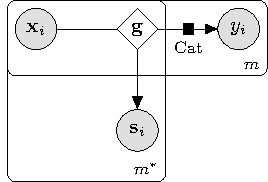
\includegraphics[width=0.35\textwidth]{results/privlearn/general_model}\label{fg:st:plate}}
\subfloat[]{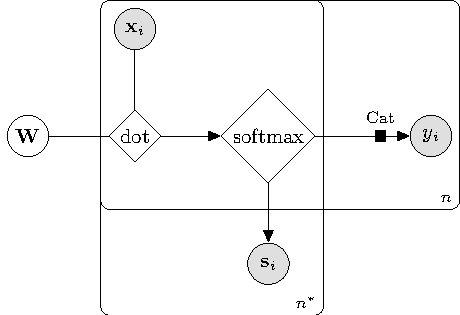
\includegraphics[width=0.35\textwidth]{results/privlearn/linear_model}\label{fg:ex:synt:plate}}
\caption{Вероятностная модель в графовой нотации: a) произвольная функция; b) линейная модель.}
\end{figure}

Для каждой реализации~$\mathbf{g}$ соответствующий блок требует уточнения. На рис.~\ref{fg:ex:synt:plate} показана более подробная реализация в случае, когда~$\mathbf{g}$~--- линейная модель.

Для задачи многоклассовой классификации рассматриваются вероятностные 
{\sl{п\,р\,е\,д\,п\,о\,л\,о\,ж\,е\,н\,и\,я:}}
\begin{enumerate}[1)]
\label{st:class:1}
	\item \emph{рассматривается функция учителя} $\mathbf{f}\in\mathfrak{F}_{\text{cl}}^{*}$~\emph{\eqref{eq:F:set:cl:priv};}
	\item \emph{рассматривается функция ученика}   $\mathbf{g}\in\mathfrak{G}_{\text{cl}}$~\emph{\eqref{eq:G:set:cl};}
	\item \emph{для истинных меток рассматривается категориальное распределение}~$p\bigr(y|\mathbf{x}, \mathbf{g}\bigr) = \text{Cat}\bigr(\mathbf{g}\bigr(\mathbf{x}\bigr)\bigr)$, \emph{где $\mathbf{g}\bigr(\mathbf{x}\bigr)$ задает вероятность каждого класса;}
	\item \emph{для меток учителя введем плотность распределения}
\begin{gather}
\label{reg:dist}
\begin{aligned}
	p\bigr(\mathbf{s}|\mathbf{x}, \mathbf{g}\bigr) = C\prod_{r=1}^{R}g_r\bigr(\mathbf{x}\bigr)^{s^r},
\end{aligned}
\end{gather}
\emph{где~$g^r$~--- вероятность класса~$r$, которую предсказывает модель ученика, а~$s^r$~--- вероятность класса~$r$, которую предсказывает модель учителя.}
\end{enumerate}
\begin{theorem}
\label{theorem:st:dist}
Пусть вероятность каждого класса отделима от нуля и единицы, т.е. для всех~$r$ выполняется условие
\begin{gather}
1 > 1- \varepsilon > g_r\bigr(\mathbf{x}\bigr) > \varepsilon > 0.
\end{gather}
Тогда при
\begin{gather}
C=\left(-1\right)^{R}\frac{R^{R/2}}{2^{R(R-1)/2}}\prod_{r=1}^{R}g_r\bigr(\mathbf{x}\bigr)\log g_r\bigr(\mathbf{x}\bigr)
\end{gather}
функция $p\bigr(\mathbf{s}|\mathbf{x}, \mathbf{g}\bigr)$, определенная в~\eqref{reg:dist}, является плотностью распределения.
\end{theorem}

Используя предположения 1--4 и подставляя в~\eqref{eq:st:12}, получаем  оптимизационную задачу:
\begin{gather}
\label{eq:st:class:1}
\begin{aligned}
\hat{\mathbf{g}} = \arg\max_{\mathbf{g}\in \mathcal{G}} & \sum_{i\not\in \mathcal{I}}\sum_{r=1}^{R}y_i^r\log g_r\bigr(\mathbf{x}_i\bigr)\bigr|_{T=1} +\\
&+ \left(1-\lambda\right)\sum_{i\in \mathcal{I}}\sum_{r=1}^{R}y_i^r\log g_r\bigr(\mathbf{x}_i\bigr)\bigr|_{T=1} + \lambda\sum_{i\in \mathcal{I}}\sum_{r=1}^{R}s_{i,r}\log g_r\bigr(\mathbf{x}_i\bigr)\bigr|_{T=T_0} +\\
&+ \lambda \sum_{i\in \mathcal{I}}\sum_{r=1}^{R}\left(\log g_r\bigr(\mathbf{x}_i\bigr)\bigr|_{T=T_0} + \log\log\frac{1}{g_r\bigr(\mathbf{x}_i\bigr)}\bigr|_{T=T_0}\right).
\end{aligned}
\end{gather}

Проанализировав выражение~\eqref{eq:st:class:1}, получаем, что первые три слагаемых совпадают со слагаемыми в выражении~\eqref{eq:hinton:1} при~$\mathcal{I} = \{1, \ldots, m\}$ и $\lambda=\frac{1}{2}$, а четвертое слагаемое является некоторым регуляризатором, который получен из вида распределения. Анализируя первые три слагаемых в выражении~\eqref{eq:st:class:1} при~$T_0 = 1$, получаем сумму кросс-энтропий между двумя распределениями для каждого объекта:
\begin{enumerate}[1)]
	\item первое распределение~--- это выпуклая комбинация с весами~$1-\lambda$ и $\lambda$ распределения, задаваемого метками объектов~$\text{Cat}\bigr(\mathbf{y}\bigr)$, и распределения, задаваемого моделью учителя~$\text{Cat}\bigr(\mathbf{s}\bigr)$;
	\item второе распределение~--- это распределение, задаваемое моделью ученика~$\text{Cat}\bigr(\mathbf{g}\bigr(\mathbf{x}\bigr)\bigr)$.
\end{enumerate}

Для задачи регрессии рассматриваются вероятностные \emph{п\,р\,е\,д\,п\,о\,л\,о\,ж\,е\,н\,и\,я:}

\begin{enumerate}[1)]
	\item \emph{рассматривается функция учителя~$\mathbf{f}\in\mathfrak{F}_{\text{rg}}^{*}$,
	\[
	\mathfrak{F}_{\text{rg}}^* = \left\{\mathbf{f}| \mathbf{f} = \mathbf{v}^*\bigr(\mathbf{x}^*\bigr), \quad \mathbf{v}^*: \mathbb{R}^{n^*} \to \mathbb{R} \right\},
	\]
	где~$\mathbf{v}^*$~--- дифференцируемая параметрическая функция;}
	\item \emph{рассматривается функция ученика~$\mathbf{g}\in\mathfrak{G}_{\text{rg}}$,
    \[
    \mathfrak{G}_{\text{rg}} = \left\{\mathbf{g}| \mathbf{g} = \mathbf{z}\bigr(\mathbf{x}\bigr), \quad \mathbf{z}: \mathbb{R}^n \to \mathbb{R}^R \right\},
    \]
    где~$\mathbf{z}$~--- дифференцируемая параметрическая функция;}
	\item \emph{истинные метки имеют нормальное распределение
	\begin{gather}
		p\bigr(y|\mathbf{x}, \mathbf{g}\bigr) = \mathcal{N}\bigr(y|\mathbf{g}\bigr(\mathbf{x}\bigr), \sigma\bigr);
	\end{gather}}
	\item \emph{метки учителя имеют распределение
	\begin{gather}
		p\bigr(s| \mathbf{x}, \mathbf{g}\bigr) = \mathcal{N}\bigr(s|\mathbf{g}\bigr(\mathbf{x}\bigr), \sigma_s\bigr).
	\end{gather}}
\end{enumerate}
Используя предположения~1--4 и подставляя в~\eqref{eq:st:12}, получаем оптимизационную задачу:
\begin{gather}
\label{eq:st:reg:1}
\begin{aligned}
\hat{g} = \arg\min_{g\in \mathcal{G}} & \sum_{i\not\in \mathcal{I}}\sigma^2\left(y_i-\mathbf{g}\bigr(\mathbf{x}_i\bigr)\right)^2 +\\
&+ \left(1-\lambda\right)\sum_{i\in \mathcal{I}}\sigma^2\left(y_i-\mathbf{g}\bigr(\mathbf{x}_i\bigr)\right)^2 + \lambda\sum_{i\in \mathcal{I}}\sigma_s^2\left(s_i-\mathbf{g}\bigr(\mathbf{x}_i\bigr)\right)^2.
\end{aligned}
\end{gather}
Выражение~\eqref{eq:st:reg:1} записано с точностью до аддитивной константы относительно~$\mathbf{g}$. 

\begin{theorem}
\label{theorem:st:reg}
Пусть множество~$\mathcal{G}$ описывает класс линейных функций вида~$\mathbf{g}\bigr(\mathbf{x}\bigr) = \mathbf{w}^{\mathsf{T}}\mathbf{x}.$ Тогда решение оптимизационной задачи~\eqref{eq:st:reg:1} эквивалентно решению задачи линейной регрессии:
\begin{gather}
\label{eq:st:reg:th:st:1}
\begin{aligned}
\mathbf{y''} = \mathbf{X}\mathbf{w} + \bm{\varepsilon},\qquad \bm{\varepsilon} \sim \mathcal{N}\bigr(\mathbf{0}, \bm{\Sigma}\bigr),
\end{aligned}
\end{gather}
где $\bm{\Sigma}^{-1}={\text{\normalfont{diag}}}\bigr(\bm{\sigma'}\bigr)$ и $\mathbf{y''}$ имеют вид:
\begin{gather}
\label{eq:st:reg:th:st:2}
\begin{aligned}
\sigma'_{i} &= \begin{cases}
\sigma^2,~\text{если}~i \not \in \mathcal{I},\\
\left(1-\lambda\right)\sigma^2+\lambda\sigma_s^2,~\text{иначе},\\
\end{cases}\\
\mathbf{y''} &= \bm{\Sigma}\mathbf{y'},\\
y'_i &= \begin{cases}
\sigma^2y_i,~\text{если}~i \not \in \mathcal{I},\\
\left(1-\lambda\right)\sigma^2y_i+\lambda\sigma_s^2s_i,~\text{иначе}.\\
\end{cases}
\end{aligned}
\end{gather}
\end{theorem}

В~\textbf{главе~3} представлен подход байесовской дистилляции. Предлагается подход, основанный на последовательном выравнивании пространств параметров модели ученика и учителя. 
\begin{definition}
\label{def:structure}
Структура модели --- упорядоченный набор структурных параметров модели, которые задают вид суперпозиции.
\end{definition}
\begin{definition}
\label{def:sopos}
Выравнивание параметрических моделей --- изменение структуры модели (одной или нескольких моделей) в результате которого векторы параметров различных моделей лежат в одном пространстве.
\end{definition}

Задана модель учителя в виде суперпозиций линейных и нелинейных преобразований:
\[
\label{ch:3:eq:st:2}
\begin{aligned}
f = \bm{\sigma} \circ \mathbf{U}_T \bm{\sigma} \circ \mathbf{U}_{T-1}\circ \ldots  \mathbf{U}_2\bm{\sigma} \circ \mathbf{U}_1,
\end{aligned}
\]
где $T$ --- число слоев модели учителя, $\bm{\sigma}$ --- функция активации, а $\mathbf{U}_t$ обозначает матрицу линейного преобразования. Матрицы $\mathbf{U}$ соединяются в вектор параметров $\mathbf{u}$ модели учителя $f$:
\[
\label{ch:3:eq:st:2.1}
\begin{aligned}
\mathbf{u} = \text{vec}\bigr(\left[\mathbf{U}_T, \mathbf{U}_{T-1}, \ldots \mathbf{U}_1\right]\bigr),
\end{aligned}
\]
где $\text{vec}$ операция векторизации соединенных матриц.
Каждая матрица $\mathbf{U}_t$ имеет размер $n_t\times n_{t-1},$ где $n_0=n,$ а  $n_T={1}$ для задачи регрессии и $n_T=R$ для задачи классификации на $R$ классов. Для построения вектора параметров $\mathbf{u}$ задается полный порядок на элементов матриц $\mathbf{U}_t$.

Пусть для вектора параметров учителя $f$ известно апостериорное распределение параметров $p\bigr(\mathbf{u}|\mathfrak{D}\bigr)$. 
На основе выборки $\mathfrak{D}$ и апостериорного распределения параметров учителя $f$ требуется выбрать модель ученика из параметрического семейства функций:
\[
\label{ch:3:eq:st:5}
\begin{aligned}
g = \bm{\sigma} \circ \mathbf{W}_L\bm{\sigma}  \circ \ldots \circ \mathbf{W}_1, \quad \mathbf{W}_l \in \mathbb{R}^{n_l \times n_{l-1}},
\end{aligned}
\]
где $L$ число слоев модели ученика.
Модель $g$ задается своим вектором параметров $\mathbf{w}$.
Следовательно, задача выбора модели $g$ эквивалентна задаче оптимизации вектора параметров $\mathbf{w}\in\mathbb{R}^{N_{\text{st}}}$.

Параметры $\hat{\mathbf{w}} \in \mathbb{R}^{N_{\text{st}}}$ оптимизируются при помощи вариационного вывода на основе совместного правдоподобия модели и данных:
\[
\label{ch:3:eq:st:6}
\begin{aligned}
\mathcal{L}\bigr(\mathfrak{D}, \mathbf{A}\bigr) = \log p\bigr(\mathfrak{D}|\mathbf{A}\bigr) = \log \int_{\mathbf{w} \in \mathbb{R}^{N_{\text{st}}}}p\bigr(\mathfrak{D}|\mathbf{w}\bigr)p\bigr(\mathbf{w}|\mathbf{A}\bigr)d\mathbf{w},
\end{aligned}
\]
где $p\bigr(\mathbf{w}| \mathbf{A}\bigr)$ --- априорное распределение вектора параметров модели ученика.
Так как взятие интеграла \eqref{ch:3:eq:st:6} является вычислительно сложной задачей, используется вариационный вывод. Для этого задается вариационное распределение параметров модели ученика $q\bigr(\mathbf{w}|\bm{\mu}, \bm{\Sigma}\bigr),$ которое аппроксимирует неизвестное апостериорное распределение $p\bigr(\mathbf{w}|\mathfrak{D}\bigr).$
Оптимизация параметров $\mathbf{w}$ сводится к решению  задачи:
\[
\label{ch:3:eq:st:7}
\begin{aligned}
\hat{\mathbf{w}} = \arg \min_{\bm{\mu}, \bm{\Sigma}, \mathbf{w}} \text{D}_{\text{KL}}\bigr(q\bigr(\mathbf{w}|\bm{\mu}, \bm{\Sigma}\bigr)||p\bigr(\mathbf{w}|\mathbf{A}\bigr)\bigr) - \log p\bigr(\mathbf{y}|\mathbf{X}, \mathbf{w}\bigr).
\end{aligned}
\]
Выражение~\eqref{ch:3:eq:st:7} не учитывает параметры учителя $f\bigr(\mathbf{x}, \mathbf{u}\bigr)$. Для использования параметров учителя при решении оптимизационной задачи\eqref{ch:3:eq:st:7} предлагается рассмотреть зависимость параметров априорного распределения $p\bigr(\mathbf{w}|\mathbf{A}\bigr)$ от параметров апостериорного распределения учителя $p\bigr(\mathbf{u}|\mathfrak{D}\bigr)$.

Апостериорное распределение параметров модели учителя предполагается нормальным:
\[
\label{ch:3:eq:ap:1}
\begin{aligned}
p\bigr(\mathbf{u}|\mathfrak{D}\bigr) = \mathcal{N}\bigr(\mathbf{m}, \bm{\Sigma}\bigr),
\end{aligned}
\]
где $\mathbf{m}$ и $\bm{\Sigma}$ параметры этого распределения. На основе параметров $\mathbf{m}$ и $\bm{\Sigma}$ требуется задать параметры $\mathbf{A}$ априорного распределения $p\bigr(\mathbf{w}|\mathbf{A}\bigr).$
Структуры моделей учителя и ученика задаются числом слоев и размером этих слоев, то возможны варианты: 1) число слоев и размер каждого слоя совпадает; 2) число слоев совпадает, а размеры различаются; 3) не совпадает число слоев.

Рассмотрим условия:
\begin{enumerate}[1)]
    \item число слоев модели учителя равняется числу слоев модели ученика $L=T$;
    \item размеры соответствующих слоев совпадают, другими словами, для всех $t, l$ таких, что $t=l$ выполняется $n_l = n_t,$ где $n_t$ обозначает размер $t$-го слоя учителя, а $n_l$ размер $l$-го слоя ученика.
\end{enumerate}
При выполнении этих условий, априорное распределение параметров модели ученика приравнивается к апостериорному распределения параметров учителя $p\bigr(\mathbf{w}|\mathbf{A}\bigr) = p\bigr(\mathbf{u}|\mathfrak{D}\bigr)$.


Проведем выравнивание модели учителя и модели ученика, согласно определению \ref{def:sopos} при помощи последовательных преобразований параметров $\mathbf{u}$. Рассмотрим преобразование
\[
\label{ch:3:eq:ap:2}
\begin{aligned}
\bm{\phi}\bigr(t, \mathbf{u}\bigr) : \mathbb{R}^{N_{\text{tr}}} \to \mathbb{R}^{N_{\text{tr}}-2n_t}
\end{aligned}
\]
вектора $\mathbf{u},$ которое описывает удаление одного нейрона из $t$-го слоя учителя.
Обозначим новый вектор параметров $\bm{\upsilon} =  \bm{\phi}\bigr(t, \mathbf{u}\bigr),$ а элементы вектора, которые удалены как $\bar{\bm{\upsilon}}.$ Заметим, что векторы $\bm{\upsilon}$ и $\bar{\bm{\upsilon}}$ являются случайными величинами. 

\begin{theorem}
Пусть задано распределение вектора параметров~$p\bigr(\mathbf{u}\bigr).$ Тогда распределение вектора параметров~$p\bigr(\bm{\upsilon}\bigr)$ представимо в виде:
\[
p\bigr(\bm{\upsilon}\bigr)  = \int\limits_{ \bm{\nu}_2 \in \mathbb{R}^{n_{t-1}}}p\bigr(\bar{\bm{\nu}}_1|\mathfrak{D}, \bm{\nu}_1=\mathbf{0}\bigr) d \bm{\nu}_2.
\]
\end{theorem}

\begin{theorem}
\label{theorem:ap:neural}
Пусть выполняются условия:
\begin{enumerate}[1)]
\item апостериорное распределение параметров $p\bigr(\mathbf{u}|\mathfrak{D}\bigr) = \mathcal{N}\bigr(\mathbf{m}, \bm{\Sigma}\bigr),$
\item число слоев модели учителя равняется числу слоев модели ученика $T=L$,
\item размеры соответствующих слоев не совпадают, другими словами, для всех $t, l,$ таких что $t=l,$ выполняется $n_t \geq n_l.$
\end{enumerate}
Тогда распределение параметров~$p\bigr(\bm{\upsilon}|\mathfrak{D}\bigr)$ также является нормальным.
\end{theorem}

Рассмотрим преобразование:
\[
\label{ch:3:eq:ap:4}
\begin{aligned}
\bm{\psi}\bigr(t, \mathbf{u}\bigr) : \mathbb{R}^{N_{\text{tr}}} \to \mathbb{R}^{N_{\text{tr}}-n_tn_{t-1}}
\end{aligned}
\]
вектора $\mathbf{u}$ которое описывает удаление одного $t$-го слоя.
Обозначим новый вектор параметров $\bm{\upsilon} = \bm{\psi}\bigr(t, \mathbf{u}\bigr),$ а элементы вектора, которые удалены как $\bar{\bm{\upsilon}}.$ 

\begin{theorem}
\label{theorem:ap:layer}
Пусть выполняются условия:
\begin{enumerate}[1)]
\item апостериорное распределение параметров $p\bigr(\mathbf{u}|\mathfrak{D}\bigr) = \mathcal{N}\bigr(\mathbf{m}, \bm{\Sigma}\bigr),$
\item соответствующие размеры слоев совпадают, $n_t=n_{t-1},$ т.е. матрица~$\mathbf{U}_t$ является квадратной,
\item функция активации удовлетворяет свойству идемпотентности $\bm{\sigma} \circ \bm{\sigma} = \bm{\sigma}$.
\end{enumerate}
Тогда апостериорное распределение также описывается нормальным распределением с плотностью распределения
\[
\label{ch:3:eq:ap:5}
\begin{aligned}
p\bigr(\bm{\upsilon}|\mathfrak{D}\bigr) = \mathcal{N}\bigr(\mathbf{m}_{\bm{\upsilon}}+\bm{\Sigma}_{\bm{\upsilon},\bar{\bm{\upsilon}}} \bm{\Sigma}_{\bar{\bm{\upsilon}},\bar{\bm{\upsilon}}}^{-1} \left(\mathbf{i} - \bar{\bm{\upsilon}}\right), \bm{\Sigma}_{\bm{\upsilon},\bm{\upsilon}} - \bm{\Sigma}_{\bm{\upsilon},\bar{\bm{\upsilon}}}\bm{\Sigma}_{\bar{\bm{\upsilon}},\bar{\bm{\upsilon}}}^{-1}\bm{\Sigma}_{\bm{\upsilon},\bar{\bm{\upsilon}}}\bigr),
\end{aligned}
\]
где
\[
\mathbf{i}=[\underbrace{1, 0, \ldots, 0}_{n_t}, \underbrace{0, 1, \ldots, 0}_{n_t}, \underbrace{0, 0, 1, \ldots, 0}_{n_t}, \underbrace{0, \ldots, 1}_{n_t}]^{\mathsf{T}}.
\]
\end{theorem}
Теорема \ref{theorem:ap:layer} задает апостериорное распределение \eqref{ch:3:eq:ap:5} параметров после удаления слоя нейросети.

Далее рассматривается задача аппроксимации последовательности:
\[
    \left[\mathbf{x}_1, \ldots, \mathbf{x}_{q}, \ldots, \mathbf{x}_{Q}\right],
\]
где~$\mathbf{x}_{q}$~--- вектор признакового описания~$q$-го элемента последовательности. 
Структура модели RNN задается размерностью скрытых слоев~$n_1, n_2, \ldots, n_T.$ Скрытое представление~$\mathbf{h}^{q}_t$ элемента последовательности~$\mathbf{x}_{q}$ для~$t$-го слоя задается выражением:
\[
    \mathbf{h}^{q}_t = \sigma\bigr(\mathbf{U}^{1}_{t}\mathbf{h}^{q}_{t-1}+\mathbf{U}^{2}_{t}\mathbf{h}^{q-1}_{t}\bigr),
\]
где матрицы~$\left\{\mathbf{U}^{1}_{t}, \mathbf{U}^{2}_{t}\right\}_{t=1}^{T}$ задают линейные отображения в модели RNN.

Отображение
\[
\bm{\phi}_{\text{RNN}}\bigr(t, \mathbf{u}\bigr) : \mathbb{R}^{\text{p}_{\text{tr}}} \to \mathbb{R}^{\text{p}_{\text{tr}}-3n_t}
\]
задает снижение размерности пространства после~$t$-го слоя на единицу. Полученный вектор параметров после снижения размерности обозначается
\[
\bm{\upsilon} = \bm{\phi}\bigr(t, \mathbf{u}\bigr).
\]
Исходный вектор~$\mathbf{u}$ состоит из подвекторов $\bm{\nu}_2, {\bm{\nu}}_1, \bm{\upsilon},$ которые описывают удаляемые, зануляемые и оставшиеся параметры соответственно.

\begin{theorem}
Пусть задано распределение вектора параметров~$p\bigr(\mathbf{u}\bigr).$ Тогда распределение вектора параметров~$p\bigr(\bm{\upsilon}\bigr)$ представимо в виде:
\[
p\bigr(\bm{\upsilon}\bigr)  = \int\limits_{ \bm{\nu}_2 \in \mathbb{R}^{n_{t-1}}}p\bigr(\bar{\bm{\nu}}_1|\mathfrak{D}, \bm{\nu}_1=\mathbf{0}\bigr) d \bm{\nu}_2.
\]
\end{theorem}

\begin{theorem}
Пусть выполняются условия:
\begin{enumerate}
\item[1)] апостериорное распределение параметров $p\bigr(\mathbf{u}|\mathfrak{D}\bigr) = \mathcal{N}\bigr(\mathbf{m}, \bm{\Sigma}\bigr),$
\item[2)] число слоев модели учителя равняется числу слоев модели ученика $T=L$,
\item[3)] размеры соответствующих пространств не совпадают~$n_t \geq n_t.$
\end{enumerate}
Тогда распределение параметров~$p\bigr(\bm{\upsilon}|\mathfrak{D}\bigr)$ также является нормальным.
\end{theorem}

\begin{theorem}
\label{ch-3:th:rnn:later}
Пусть выполняются условия:
\begin{enumerate}
\item[1)] апостериорное распределение параметров $p\bigr(\mathbf{u}|\mathfrak{D}\bigr) = \mathcal{N}\bigr(\mathbf{m}, \bm{\Sigma}\bigr),$
\item[2)] размеры соответствующих пространств совпадают: $n_t=n_{t+1}.$
\item[3)] функция активации удовлетворяет свойству идемпотентности $\bm{\sigma} \circ \bm{\sigma} = \bm{\sigma}$.
\end{enumerate}
Тогда апостериорное распределение также описывается нормальным распределением с плотностью распределения:
\[
\begin{aligned}
p\bigr(\bm{\upsilon}|\mathfrak{D}\bigr) = \mathcal{N}\bigr(\mathbf{m}_{\bm{\upsilon}}+\bm{\Sigma}_{\bm{\upsilon},\bar{\bm{\upsilon}}} \bm{\Sigma}_{\bar{\bm{\upsilon}},\bar{\bm{\upsilon}}}^{-1} \left(\mathbf{i} - \bar{\bm{\upsilon}}\right), \bm{\Sigma}_{\bm{\upsilon},\bm{\upsilon}} - \bm{\Sigma}_{\bm{\upsilon},\bar{\bm{\upsilon}}}\bm{\Sigma}_{\bar{\bm{\upsilon}},\bar{\bm{\upsilon}}}^{-1}\bm{\Sigma}_{\bm{\upsilon},\bar{\bm{\upsilon}}}\bigr),
\end{aligned}
\]
где
\[
\mathbf{i}=[\underbrace{1, 0, \ldots, 0}_{n_t}, \underbrace{0, 1, \ldots, 0}_{n_t}, \underbrace{0, 0, 1, \ldots, 0}_{n_t}, \underbrace{0, \ldots, 1}_{n_t}, \underbrace{0, \ldots, 0}_{n_t\times n_t}]^{\mathsf{T}}.
\]
\end{theorem}

Теорема~\ref{ch-3:th:rnn:later} задает апостериорное распределение параметров после удаления одного слоя модели RNN.

Множество всех структур задается последовательностью натуральных чисел:
\[
\mathfrak{H} = \left\{(n_1, n_2, \ldots, n_{T}), \quad n_i \in \mathbb{N}, T \in \mathbb{N}\right\}.
\]
Множество структур, порождаемое структурой~$(n_{1}', n_{2}', \ldots, n_{L}')$ учителя~$\mathbf{f}$:
\[
\begin{aligned}
    \mathfrak{H}_{\mathbf{f}} = \Big\{\mathbf{n} = \left(n_1, \ldots, n_{T}\right)|~&n_i \in \mathbb{N}; \\
    & n_i \leq n_{i}',~3\leq T\leq L,~n_{T}=n^{'}_{L}; \quad n_{T-1} \leq n_{i}',~i > T\Big\},
\end{aligned}
\]
описывает конечное подмножество структур в континуальном множестве.

\begin{theorem}
\label{th-9:visual}
Для произвольной структуры~$\mathbf{n} \in \mathfrak{H}_{\mathbf{f}}$ существует последовательность локальных выравнивающих преобразований $\tau = (\ldots, \bm{\phi}, \ldots, \bm{\psi}, \ldots),$ сохраняющее распределение параметров модели~$\mathbf{f}$.
\end{theorem}

Рассмотрим теорему~\ref{th-9:visual} на примере. Учитель~$\mathbf{f}$ имеет структуру~$(10, 6, 7, 10)$, модель ученика~$\mathbf{g}$ имеет структуру~$(10,4,6,10)$.
\[
\xymatrix{
% First Line
\mathbf{f}\ar@[blue][d]_{\color{blue}\bm{\phi}\bigr(3\bigr)}\ar@[red][r]^{\color{red}\bm{\phi}\bigr(2\bigr)}
& 
\mathbf{f}_{\tau_1}'\ar@[darkcyan][d]\ar@[red][r]^{\color{red}\bm{\phi}\bigr(2\bigr)}
&
\mathbf{f}_{\tau_1}''\ar@[red][d]^{\color{red}\bm{\phi}\bigr(3\bigr)}
\\
% Second Line
\mathbf{f}_{\tau_2}'\ar@[blue][r]_{\color{blue}\bm{\phi}\bigr(2\bigr)}
& 
\mathbf{f}_{\tau_2}''\ar@[blue][r]_{\color{blue}\bm{\phi}\bigr(2\bigr)}
&
\mathbf{g}
}
\]
Построенные последовательности выравнивающих преобразований модели учителя~$\mathbf{f}$ в модель ученика $\mathbf{g}$:
\[
{\color{red}\tau_1=\left(\bm{\phi}\bigr(2\bigr), \bm{\phi}\bigr(2\bigr), \bm{\phi}\bigr(3\bigr)\right)}, {\color{blue}\tau_2=\left(\bm{\phi}\bigr(3\bigr), \bm{\phi}\bigr(2\bigr), \bm{\phi}\bigr(2\bigr)\right)}, {\color{darkcyan}\tau_3=\left(\bm{\phi}\bigr(2\bigr), \bm{\phi}\bigr(3\bigr), \bm{\phi}\bigr(2\bigr)\right)}.
\]
Цветом выделены разные последовательности преобразований.
Из примера видно, что последовательность выравнивающих преобразований существует, но не единственно. Преобразования $\bm{\phi}, \bm{\psi}$ выравнивают пространства параметров учителя~$\mathbf{f}$ и ученика~$\mathbf{g}$. После выравнивания параметрических моделей получаем, что параметры модели учителя и модели учителя принадлежат одному пространству параметров.

В~\textbf{главе~4} рассматривается методы задания априорного распределения для локальных моделей смеси экспертов.

\begin{definition}
\label{def:1}
Модель~$\mathbf{g}$ называется локальной моделью для выборки~$\textbf{U},$ если~$\mathbf{g}$ аппроксимирует некоторое не пустое подмножество~$\textbf{U}'\subset\textbf{U}$.
\end{definition}

\begin{definition}
\label{def:2}
Мультимодель~$\mathbf{f}$ называется смесью экспертов, если
\[
\label{ch4-eq:st:2}
\begin{aligned}
\mathbf{f} = \sum_{k=1}^{K}\pi_{k}\mathbf{g}_k\bigr(\mathbf{w}_k\bigr), \qquad \pi_{k}\bigr(\mathbf{x}, \mathbf{V}\bigr):\mathbb{R}^{n\times \left|\mathbf{V}\right|} \to [0, 1], \qquad \sum_{k=1}^{K}\pi_{k}\bigr(\mathbf{x}, \mathbf{V}\bigr) = 1,
\end{aligned}
\]
где~$\mathbf{g}_k$ является~$k$-й локальной моделью,~$\pi_k$ --- шлюзовая функция, вектор~$\mathbf{w}_k$ является параметрами~$k$-й локальной моделью, а~$\mathbf{V}$ --- параметры шлюзовой функции.
\end{definition}

В качестве локальных моделей рассматриваются линейные модели. В качестве шлюзовой функции рассматривается двухслойный перцептрон:
\[
\label{ch4-eq:st:3}
\begin{aligned}
\mathbf{g}_k\bigr(\textbf{x}\bigr) = \textbf{w}_k^{\mathsf{T}}\textbf{x}, \quad
\bm{\pi}\bigr(\mathbf{x}, \mathbf{V}\bigr) = \text{softmax}\bigr(\mathbf{V}_{1}^{\mathsf{T}}\bm{\sigma}\bigr(\mathbf{V}_2^{\mathsf{T}}\mathbf{x}\bigr)\bigr),
\end{aligned}
\]
где~$\mathbf{V} = \bigr\{\mathbf{V}_1, \mathbf{V}_2\bigr\}$~--- множество параметров шлюзовой функции.

Предлагается использовать вероятностный подход для описания смеси экспертов. Вводиться предположение, что~$\textbf{y}$ является случайным вектором, который задается плотностью распределения~$p\bigr(\textbf{y}|\textbf{X}\bigr)$. Предполагается, что плотность распределения~$p\bigr(\textbf{y}|\textbf{X}, \textbf{f}\bigr)$ аппроксимирует истинную плотность распределения~$p\bigr(\textbf{y}|\textbf{X}\bigr)$:
\[
\label{ch4-eq:st:new:1}
\begin{aligned}
p\bigr(\textbf{y}|\textbf{X}, \textbf{f}\bigr) = \prod_{i=1}^{N}\left(\sum_{k=1}^{K}\pi_kp_{k}\bigr(y_{i}|\textbf{g}_{k}\bigr(\mathbf{x}_{i}\bigr)\bigr)\right),
\end{aligned}
\]
где~$\textbf{f}$~--- это смесь экспертов, а~$\textbf{g}_k, \bm{\pi}$ определяются выражением \eqref{ch4-eq:st:3}.

Пусть~$\textbf{w}_k$ является случайным вектором, который задается плотностью распределения~$p^{k}\bigr(\mathbf{w}_k\bigr)$. Получим совместное распределения параметров локальных моделей и вектора ответов:
\[
\label{ch4-eq:st:4}
\begin{aligned}
p\bigr(\mathbf{y}, \mathbf{W}|\mathbf{X}, \mathbf{V}\bigr) = \prod_{k=1}^{K}p^{k}\bigr(\mathbf{w}_k\bigr)\prod_{i=1}^{N}\left(\sum_{k=1}^{K}\pi_{k}p_{k}\bigr(y_i|\mathbf{w}_k, \mathbf{x}_i\bigr)\right),
\end{aligned}
\]
где~$\mathbf{W} = \bigr\{\mathbf{w}_1, \mathbf{w}_2, \ldots, \mathbf{w}_K\bigr\}.$
Оптимальные параметры находятся при помощи максимизации правдоподобия:
\[
\label{ch4-eq:st:5}
\begin{aligned}
\hat{\mathbf{V}}, \hat{ \mathbf{W}} = \arg\max_{\mathbf{V}, \mathbf{W}} p\bigr(\mathbf{y},  \mathbf{W}|\mathbf{X}, \mathbf{V}\bigr).
\end{aligned}
\]

Для построения смеси экспертов, введены вероятностные предположения о данных:
\begin{enumerate}[1)]
	\item правдоподобие~$p_{k}\bigr(y_{i}|\mathbf{w}_{k}, \mathbf{x}_{i}\bigr) = \mathcal{N}\bigr(y_{i}|\mathbf{w}_{k}^{\mathsf{T}}\mathbf{x}_{i}, \beta^{-1}\bigr),$ где параметр~$\beta$ является уровнем шума,
	\item априорное распределение параметров~$p^{k}\bigr(\mathbf{w}_{k}\bigr) = \mathcal{N}\bigr(\mathbf{w}_{k}|\mathbf{w}^{0}_{k}, \mathbf{A}_{k}\bigr),$ где~$\mathbf{w}^{0}_{k}$~--- вектор размерности~$n\times1$, а ~$\mathbf{A}_{k}$~--- ковариационная матрица размерности~$n\times n$,
	\item регуляризация априорного распределения~$p\bigr(\bm{\varepsilon}_{k,k'}|\bm{\Xi}\bigr) = \mathcal{N}\bigr(\bm{\varepsilon}_{k,k'}|\mathbf{0},  \bm{\Xi}\bigr),$ где~$\bm{\Xi}$~--- ковариационная матрица, а~$\bm{\varepsilon}_{k,k'} = \mathbf{w}_{k}^{0}-\mathbf{w}_{k'}^{0}.$
\end{enumerate}

Используя предположения~$1), 2), 3)$ и выражение \eqref{ch4-eq:st:4} получаем полное правдоподобие:
\[
\label{ch4-eq:em:1}
\begin{aligned}
p\bigr(\mathbf{y}, \mathbf{W}|\mathbf{X}, \mathbf{V}, \textbf{A}, \textbf{W}^{0}, \bm{\Xi}, \beta\bigr) = &\prod_{i=1}^{N}\left(\sum_{k=1}^{K}\pi_{k}\mathcal{N}\bigr(y_{i}|\mathbf{w}_{k}^{\mathsf{T}}\mathbf{x}_{i}, \beta^{-1}\bigr)\right)\cdot\\
&\cdot\prod_{k=1}^{K}\mathcal{N}\bigr(\mathbf{w}_{k}|\mathbf{w}^{0}_{k}, \mathbf{A}_{k}\bigr)\cdot\prod_{k,k'=1}^{K}\mathcal{N}\bigr(\bm{\varepsilon}_{k,k'}|\mathbf{0},  \bm{\Xi}\bigr),
\end{aligned}
\]
где~$\mathbf{A} = \left\{\mathbf{A}_1, \ldots, \mathbf{A}_K\right\}.$

Функция обоснованности получается при интегрировании по параметрам~$\textbf{W}, \textbf{Z}$:
\[
\label{ch4-eq:em:3}
\begin{aligned}
\mathbf{V}, \mathbf{W}^0, \textbf{A},  \beta = \arg\max_{\mathbf{V}, \mathbf{W}^0, \textbf{A}, \beta} \int_{\textbf{W}, \textbf{Z}}\log p\bigr(\mathbf{y}, \textbf{Z}, \textbf{W}|\mathbf{X}, \mathbf{V}, \textbf{A}, \textbf{W}^{0}, \bm{\Xi}, \beta\bigr)d\textbf{W}d\textbf{Z}.
\end{aligned}
\]
Рассмотрим вариационную плотность~$q\bigr(\textbf{W}, \textbf{Z}\bigr)$ для параметров~$\textbf{W}, \textbf{Z}$. Тогда функция обоснованности принимает вид:
\[
\label{ch4-eq:em:new:1}
\begin{aligned}
\log p&\bigr(\mathbf{y}|\mathbf{X}, \mathbf{V}, \textbf{A}, \textbf{W}^{0}, \bm{\Xi}, \beta\bigr) =\\
&=\mathcal{L}\bigr(q, \textbf{V}, \textbf{W}^{0}, \textbf{A}, \beta\bigr)+\mathsf{D}_{KL}\left(q\bigr(\textbf{W}, \textbf{Z}\bigr)||p\bigr(\textbf{W}, \textbf{Z}|\mathbf{y}, \mathbf{X}, \mathbf{V}, \textbf{A}, \textbf{W}^{0}, \bm{\Xi}, \beta\bigr)\right)
\end{aligned}
\]
Используя \eqref{ch4-eq:em:new:1} получаем нижнюю оценку обоснованости:
\[
\label{ch4-eq:em:new:2}
\begin{aligned}
\log p\bigr(\mathbf{y}|\mathbf{X}, \mathbf{V}, \textbf{A}, \textbf{W}^{0}, \bm{\Xi}, \beta\bigr)\geq \mathcal{L}\bigr(q, \textbf{V}, \textbf{W}^{0}, \textbf{A}, \beta\bigr),
\end{aligned}
\]
где~$\mathcal{L}\bigr(q, \textbf{V}, \textbf{W}^{0}, \textbf{A}, \beta\bigr)$ называется нижней оценкой обоснованности.

Используем EM--алгоритм для решения оптимизационной задачи \eqref{ch4-eq:em:3}. EM--алгоритм вместо оптимизации~$\log p\bigr(\mathbf{y}|\mathbf{X}, \mathbf{V}, \textbf{A}, \textbf{W}^{0}, \bm{\Xi}, \beta\bigr)$ оптимизирует нижнюю оценку~$\mathcal{L}\left(q, \textbf{V}, \textbf{W}^{0}, \textbf{A}, \beta\right)$.


Сначала решается оптимизационная задача:
\[
\label{ch4-eq:em:new:3}
\begin{aligned}
\mathcal{L}\bigr(q, \textbf{V}, \textbf{W}^{0}, \textbf{A}, \beta\bigr) \to \max_{q\bigr(\textbf{W}, \textbf{Z}\bigr)},
\end{aligned}
\]
где параметры~$\textbf{V}, \textbf{W}^{0}, \textbf{A}, \beta$ являются зафиксированными.

Пусть совместное распределение~$q\bigr(\mathbf{Z}, \mathbf{W}\bigr)$ удовлетворяет условию независимости~$q\bigr(\mathbf{Z}, \mathbf{W}\bigr) = q\bigr(\mathbf{Z}\bigr)q\bigr(\mathbf{W}\bigr)$. 
Далее символом~$\propto$ обозначим то, что обе стороны выражения равны с точностью до аддитивной константы.
Сначала находится распределение~$q\bigr(\textbf{Z}\bigr)$:
\[
\label{ch4-eq:em:4}
\begin{aligned}
p\bigr(z_{ik} = 1\bigr) = \frac{\exp\bigr(\log\pi_{k}\bigr(\textbf{x}_{i}, \textbf{V}\bigr) - \frac{\beta}{2}\left(\textbf{x}_{i}^{\mathsf{T}}\mathsf{E}\textbf{w}_{k}\textbf{w}_{k}^{\mathsf{T}}\textbf{x}_{i} - \textbf{x}_{i}^{\mathsf{T}}\mathsf{E}\textbf{w}_{k}\right)\bigr)}{\sum_{k'=1}^{K}\exp\bigr(\log\pi_{k'}\bigr(\textbf{x}_{i}, \textbf{V}\bigr) - \frac{\beta}{2}\left(\textbf{x}_{i}^{\mathsf{T}}\mathsf{E}\textbf{w}_{k'}\textbf{w}_{k'}^{\mathsf{T}}\textbf{x}_{i} - \textbf{x}_{i}^{\mathsf{T}}\mathsf{E}\textbf{w}_{k'}\right)\bigr)}.
\end{aligned}
\]
Используя выражения \eqref{ch4-eq:em:4} получаем, что распределение~$q\bigr(z_{ik}\bigr)$ является бернулевским распределением с параметром~$z_{ik},$ которое задается выражением \eqref{ch4-eq:em:4}.
Далее найдем распределение~$q\bigr(\textbf{W}\bigr)$:
\[
\label{ch4-eq:em:5}
\begin{aligned}
\log q\bigr(\textbf{W}\bigr) &\propto \sum_{i=1}^{N}\sum_{k=1}^{K}\mathsf{E}z_{ik}\left[\log\pi_{k}\bigr(\textbf{x}_{i, \textbf{V}}\bigr) - \frac{\beta}{2}\left(y_{i} - \textbf{w}_{k}^{\mathsf{T}}\textbf{x}_{i}\right)^{2} + \frac{1}{2}\log\frac{\beta}{2\pi}\right] + \\
&+ \sum_{k=1}^{K}\left[-\frac{1}{2}\left(\textbf{w}_{k} - \textbf{w}_{k}^{0}\right)^{\mathsf{T}}\textbf{A}_{k}^{-1}\left(\textbf{w}_{k} - \textbf{w}_{k}^{0}\right) + \frac{1}{2}\log\det\textbf{A}^{-1}_{k} - \frac{n}{2}\log2\pi\right] \\
&\propto \sum_{k=1}^{K}\left[\textbf{w}_{k}^{\mathsf{T}}\left(\textbf{A}_{k}^{-1}\textbf{w}_{k}^{0}+\beta\sum_{i=1}^{N}\textbf{x}_{i}y_{i}\mathsf{E}z_{ik}\right)-\frac{1}{2}\textbf{w}_{k}^{\mathsf{T}}\left(\textbf{A}_{k}^{-1}+\beta\sum_{i=1}^{N}\textbf{x}_{i}\textbf{x}_{i}^{\mathsf{T}}\right)\textbf{w}_{k}\right].
\end{aligned}
\]
Используя выражение \eqref{ch4-eq:em:5} получаем, что  распределение~$q\bigr(\mathbf{w}_{k}\bigr)$ является нормальным распределением со средним~$\mathbf{m}_{k}$ и ковариационной матрицей~$\mathbf{B}_k$:
\[
\label{ch4-eq:em:6}
\begin{aligned}
\mathbf{m}_{k} = \mathbf{B}_{k}\left(\mathbf{A}_{k}^{-1}\mathbf{w}_{k}^{0}+\beta\sum_{i=1}^{N}\mathbf{x}_{i}y_{i}\mathsf{E}z_{ik}\right), \qquad \mathbf{B}_{k} = \left(\mathbf{A}_{k}^{-1}+\beta\sum_{i=1}^{N}\mathbf{x}_{i}\mathbf{x}_{i}^{\mathsf{T}}\mathsf{E}z_{ik}\right)^{-1}.
\end{aligned}
\]

Далее решается оптимизационная задача:
\[
\label{ch4-eq:em:new:3}
\begin{aligned}
\mathcal{L}\bigr(q, \textbf{V}, \textbf{W}^{0}, \textbf{A}, \beta\bigr) \to \max_{\textbf{V}, \textbf{W}^{0}, \textbf{A}, \beta},
\end{aligned}
\]
где~$q\bigr(\textbf{W}, \textbf{Z}\bigr)$ является известной плотностью распределения.
Распределение~$q\bigr(\mathbf{Z}, \mathbf{W}\bigr)$ является фиксированным, в то время как вариацонная нижняя оценка~$\mathcal{L}\bigr(\textbf{V}, \textbf{W}^{0}, \textbf{A}, \beta\bigr)$ максимизируется по параметрам~$\mathbf{V}, \mathbf{W}^0, \textbf{A},  \beta$:
\[
\label{ch4-eq:em:7}
\begin{aligned}
\mathcal{L}&\bigr(\textbf{V}, \textbf{W}^{0}, \textbf{A}, \beta\bigr) = \sum_{i=1}^{N}\sum_{k=1}^{K}\mathsf{E}z_{ik}\left[\log\pi_k\bigr(\textbf{x}_i, \textbf{V}\bigr) - \frac{\beta}{2}\mathsf{E}\left(y_{i} - \textbf{w}_{k}^{\mathsf{T}}\textbf{x}_{i}\right)^{2} + \frac{1}{2}\log\frac{\beta}{2\pi}\right] +\\
&+ \sum_{k=1}^{K}\left[-\frac{1}{2}\mathsf{E}\left(\textbf{w}_{k} - \textbf{w}_{k}^{0}\right)^{\mathsf{T}}\textbf{A}_{k}^{-1}\left(\textbf{w}_{k} - \textbf{w}_{k}^{0}\right) + \frac{1}{2}\log\det\textbf{A}^{-1}_{k} - \frac{n}{2}\log2\pi\right] +\\
&+ \sum_{k=1}^{K}\sum_{k'=1}^{K}\left[-\frac{1}{2}\left(\textbf{w}_{k}^{0}-\textbf{w}_{k'}^{0}\right)^{\mathsf{T}}\bm{\Xi}^{-1}\left(\textbf{w}_{k}^{0}-\textbf{w}_{k'}^{0}\right) +\frac{1}{2}\log\det\bm{\Xi} -\frac{n}{2}\log{2\pi}\right].
\end{aligned}
\]
Получены оптимальное значения параметров~$\textbf{A}_{k}, \beta$ и для параметров~$\textbf{w}_{k}^{0}:$
\[
\label{ch4-eq:em:9}
\begin{aligned}
\textbf{A}_{k} &= \mathsf{E}\textbf{w}_{k}\textbf{w}_{k}^{\mathsf{T}} - \textbf{w}_{k}^{0}\mathsf{E}\textbf{w}_{k}^{\mathsf{T}} - \mathsf{E}\textbf{w}_{k}\textbf{w}_{k}^{0\mathsf{T}} + \textbf{w}_{k}^{0}\textbf{w}_{k}^{0\mathsf{T}},\\
\frac{1}{\beta} &= \frac{1}{N}\sum_{i=1}^{N}\sum_{k=1}^{K}\left[y_{i}^{2}-2y_{i}\textbf{x}_{i}^{\mathsf{T}}\mathsf{E}\textbf{w}_{k} + \textbf{x}_{i}^{\mathsf{T}}\mathsf{E}\textbf{w}_{k}\textbf{w}_{k}^{\mathsf{T}}\textbf{x}_{i}\right]\mathsf{E}z_{ik}\\
\textbf{w}_{k}^{0} &= \left[\textbf{A}_{k}^{-1}+\left(K-1\right)\bm{\Xi}\right]^{-1}\left(\textbf{A}^{-1}_{k}\mathsf{E}\textbf{w}_{k}+\bm{\Xi}\sum_{k'=1, k'\not=k}^{K}\textbf{w}_{k'}^{0}\right).
\end{aligned}
\]
Получаем итеративную процедуру, которая сходится к некоторому локальному максимуму оптимизационной задачи \eqref{ch4-eq:em:3}.

В~\textbf{главе~5} рассмотрены методы для задания порядка на множестве параметров нейросетевых моделей.

Предлагается метод основанный на модификации метода Белсли. Пусть $\textbf{w}$~--- вектор параметров доставляющий минимум функционалу потерь $\mathcal{L},$ а $\textbf{A}_\text{ps}$ соответствующая ему ковариационная матрица.

Выполним сингулярное разложение матрицы
\[
\textbf{A}_\text{ps} = \textbf{U}{\bf\Lambda}\textbf{V}^\mathsf{T}.
\]
Индекс обусловленности $\eta_{j}$ определим как отношение максимального элемента к $j$-му элементу матрицы ${\bf\Lambda}$. Для нахождения мультиколлинеарных признаков требуется найти индекс $\xi$ вида:
\[
\xi = \arg\max_{j\in \mathcal{A}}{\eta_j}.
\]

Дисперсионный долевой коэффициент $q_{ij}$ определим как вклад $j$-го признака в дисперсию $i$-го элемента вектора параметра $\textbf{w}$:
\[
q_{ij} = \frac{u^2_{ij}/\lambda_{jj}}{\sum^n_{j=1}{u^2_{ij}/\lambda_{jj}}}.
\]

Большие значение дисперсионных долей указывают на наличие зависимости между параметрами. Находим долевые коэффициенты, которые вносят максимальный вклад в дисперсию параметра $w_\xi$:
\[
\zeta = \arg\max_{j\in \mathcal{A}}{q_{\xi j}}.
\]
Параметр с индексом $\zeta$ определим как наименее релевантный параметр нейросети.

В~\textbf{главе~6} продемонстрировано применение предложенных методов к прикладным задачам классификации и регрессии, а также для задач выбора оптимального размера выборки, а также к задаче классификации временных рядов.

В \textbf{заключении} представлены основные результаты диссертационной работы.
\begin{enumerate}
    \item Предложен байесовский метод выбора моделей с использованием модели учителя с привилегированной и накопленной информации.
    \item Доказаны теоремы о свойствах дистилляции, 
    \begin{itemize}
        \item[---] \emph{теоремы об эквивалентности} для дистилляции моделей в случае задачи регрессии и классификации,
        \item[---] \emph{теоремы о виде априорного распределения} параметров модели ученика в байесовской дистилляции.
    \end{itemize}
    \item Предложен метод выравнивания структур параметрических моделей. Предложен метод выбора априорного распределения параметров модели ученика с использованием апостериорного распределения параметров модели учителя для случаев
    \begin{itemize}
        \item[---] различных размерностей пространств параметров отдельных слоев,
        \item[---] различного в числа слоев нескольких моделей.
    \end{itemize}
    \item Предложены методы задания порядка на множестве параметров моделей
    \begin{itemize}
        \item[---] на основе корреляции параметров,
        \item[---] на основе оценки скорости сходимости параметров.
    \end{itemize}
    \item Предложена вероятностная интерпретации дистилляции моделей глубокого обучения. Исследованы свойства дистилляции моделей глубокого обучения.
\end{enumerate}

\textbf{Публикации соискателя по теме диссертации}

Публикации в журналах ВАК
\begin{enumerate}
    \item \textit{Грабовой А.В., Стрижов В.В.} Байесовская дистилляция моделей глубокого обучения~// Автоматика и телемеханика, 2021.
    \item \textit{Грабовой А.В., Стрижов В.В.} Анализ выбора априорного распределения для смеси экспертов~// Журнал вычислительной математики и математической физики, 2021.
    \item \textit{A. Grabovoy, V. Strijov.} Quasi-periodic time series clustering for human // Lobachevskii Journal of Mathematics, 2020.
    \item \textit{Грабовой А.В., Бахтеев О. Ю., Стрижов В.В.} Введение отношения порядка на множестве параметров аппроксимирующих моделей~// Информатика и ее применения, 2020.
    \item \textit{Грабовой А.В., Бахтеев О.Ю., Стрижов В.В.} Определение релевантности параметров нейросети~// Информатика и ее применения, 2019.
    \item \textit{Грабовой\;А.В., Стрижов\;В.В.} Вероятностная интерпретация задачи дистилляции~// Автоматика и телемеханика, 2022.
\end{enumerate}

\end{document}